\documentclass[26pt, paperwidth=36in,paperheight=48in]{tikzposter} % See Section 3
\tikzposterlatexaffectionproofoff
\usepackage{helvet}
\renewcommand{\familydefault}{\sfdefault}
\usepackage[T1]{fontenc}
\usepackage{braket}
\usepackage{subcaption}
\usepackage{graphicx}
\usepackage{calc}
\usepackage[export]{adjustbox}
\usepackage[outline]{contour}
\usepackage{mathtools}




\newcommand{\myfont}{\fontsize{26}{40}\selectfont}
\newcommand{\mysmallerfont}{\fontsize{20}{34}\selectfont}

% title stuff
\makeatletter
\def\title#1{\gdef\@title{\scalebox{\TP@titletextscale}{%
			\begin{minipage}[t]{\linewidth}
				\centering
				#1
				\par
				\vspace{-0.65cm}
			\end{minipage}%
}}}
\makeatother


\title{
	\fontsize{70}{80} \selectfont {Spin-Imbalanced Unitary Fermi Gas \\ \vspace{0.7cm} in a Uniform Trapping Potential}
}

\author{
	\fontsize{36}{50} \selectfont Eric Wolf, Huan Q Bui, Martin Zwierlein} 
\institute{
	\fontsize{36}{70} \selectfont MIT-Harvard Center for Ultracold Atoms, Research Laboratory of Electronics,\\\vspace{20pt}Massachusetts Institute of Technology, Cambridge, MA 02139} % See Section 4.1


\makeatletter
\renewcommand\TP@maketitle{\centering
	\begin{minipage}{0.15\linewidth}%
		\vspace{-10pt}
		
\includegraphics[width=\textwidth]{figures/header/cua-logo.pdf}
	\end{minipage}%
	\hspace{5.9cm}
	\begin{minipage}{0.55\linewidth}\centering
		\color{titlefgcolor}
		\vspace{20pt}
		{\@title \par}
	\end{minipage}\hfill
	\begin{minipage}{0.21\linewidth}
		\vspace{-10pt}
		
\includegraphics[width=\textwidth]{figures/header/mit.eps}
	\end{minipage}%
	\vspace*{70pt}
	{\huge \@author \par}
	\vspace*{0pt}
	{\LARGE \@institute}%
}%
\makeatother

%%% end of title stuff


\usetheme{Default} % See Section 5
\usecolorpalette{Default}
\useblockstyle{Default}
\definecolor{BEC1blue}{rgb}{0, 0.14,0.5}
\definecolor{BEC1grey}{rgb}{0.86, 0.86, 0.86}
\colorlet{backgroundcolor}{BEC1blue}
\colorlet{framecolor}{white}
\colorlet{titlebgcolor}{white}
\colorlet{notefrcolor}{white} 
\colorlet{noteframecolor}{white} 
\colorlet{notebgcolor}{white}


\definebackgroundstyle{BEC1}{
	\draw[line width=0pt, 
	left color = backgroundcolor, 
	right color    = backgroundcolor!60!white] (bottomleft) rectangle (topright);
}

\usebackgroundstyle{BEC1}


\usepackage{blindtext}
\usepackage{comment}






\begin{document}
	
\maketitle[width=0.96\textwidth, roundedcorners=0] % See Section 4.1


%% first row
\begin{columns} % See Section 4.4
\column{0.4}
\colorlet{blocktitlebgcolor}{BEC1grey}
\block[roundedcorners=0]{\textcolor{BEC1blue}{Unitary Fermi Gas in a Box Potential}}
{

\begin{minipage}{0.18\textwidth}
	\flushleft
	\vspace{0.5cm}
	\textbf{Unitary Fermi Gas}
	\vspace{0.5cm}
	\myfont
	\begin{itemize}
		
		\item Relevant to systems ranging from neutron stars to high-${T_c}$ superconductors
		
		\item Unitary Fermi gas is scale-invariant
				
		\item Realize unitarity with $\ket{1} - \ket{3}$ Feshbach resonance in $^6$Li
		
		\item Realize spin-imbalance with imperfect LZ RF transfer
		
		\item Evaporatively cool spin mixture to below $T_F$
	\end{itemize}
\vspace{1.5cm}
\end{minipage}
\hspace{0.7cm}
\begin{minipage}{0.15\textwidth}
	\begin{minipage}{\textwidth}
		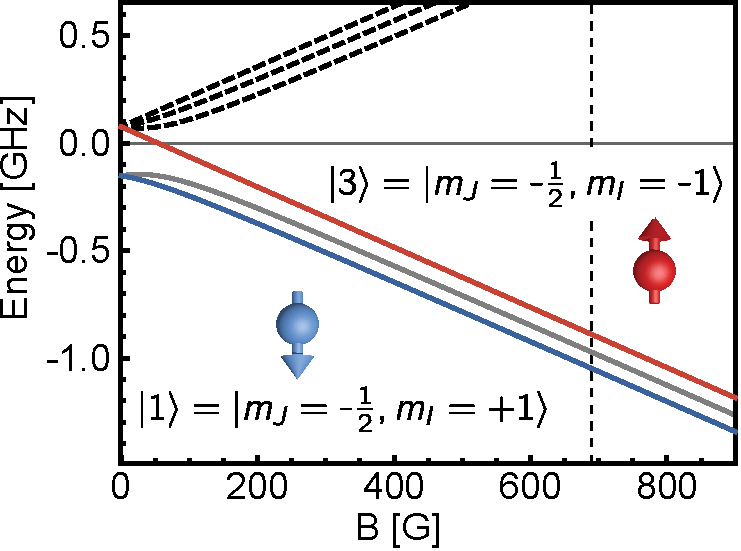
\includegraphics[width=1\textwidth]{figures/BreitRabiLi6.pdf}
	\end{minipage}
	
	\vspace{0.5cm}
	\hspace{-2cm}
	\begin{minipage}{\textwidth}
		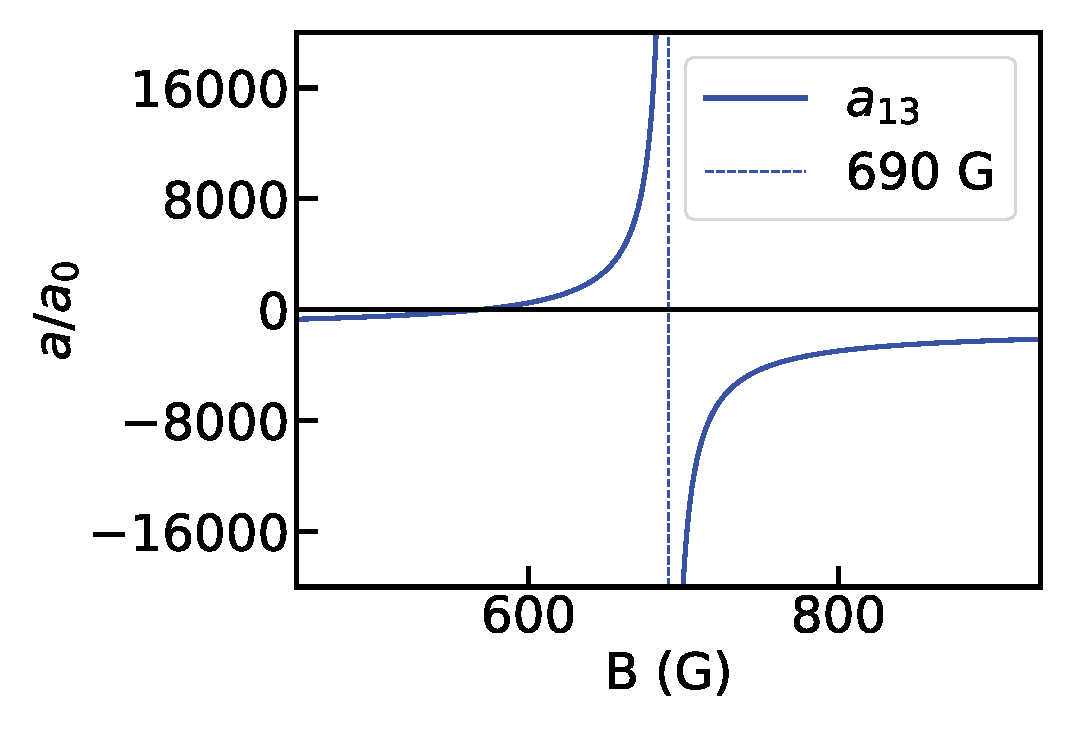
\includegraphics[width=1.15\textwidth]{figures/Feshbach_Plot_Redone.eps}
	\end{minipage}
\end{minipage}


%%%%

\vspace{0.5cm}
\begin{minipage}{0.14\textwidth}
	\flushleft
	\textbf{Box Potential [1]}
	\vspace{0.5cm}
	\myfont
	\begin{itemize}
		\item Hollow blue-detuned beams realize (quasi) flat potential
		
		\item Reduces influence of trap averaging \& targets smaller range of densities
		
		\item Momentum imaging possible via residual axial harmonic trap
	\end{itemize}
\end{minipage}
\hspace{-0.5cm}
\begin{minipage}{0.15\textwidth}
	\centering
	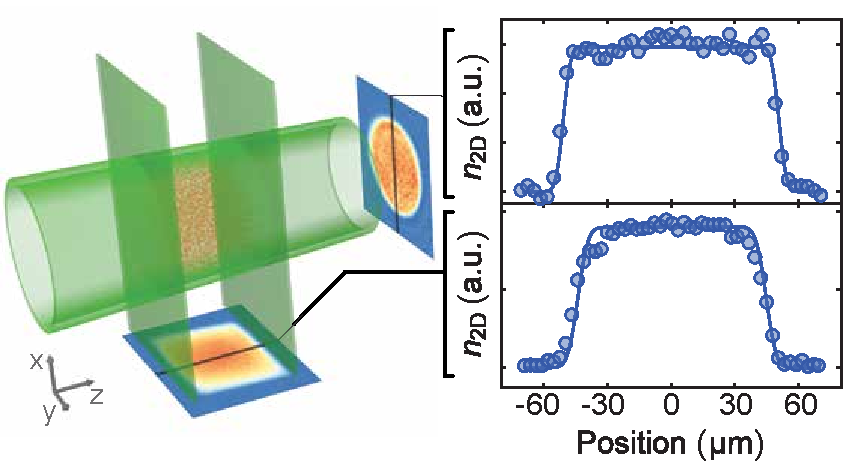
\includegraphics[scale=1.25]{figures/box_cartoon.pdf}
\end{minipage}
\vspace{2.48cm}

} 







%%%%%% 

\column{0.6}
\colorlet{blocktitlebgcolor}{BEC1grey}
\block[roundedcorners=0]{\textcolor{BEC1blue}{Imaging Optically Dense Atomic Clouds}}
{
	\begin{minipage}{0.26\textwidth}
		\flushleft
		\vspace{0.5cm}
		\textbf{Polarization Rotation Imaging (PRI) [2, 3, 4]}
		\vspace{0.5cm}
		\myfont
		\begin{itemize}
		\item Phase shift + absorption of detuned imaging light $\rightarrow$ atomic density	
		\item Orthogonal polarizations $\ket{H}$ and $\ket{V}$. Only $\ket{H}$ interacts with the atoms
		\item Atoms act on imaging light as 
		$$ A = \left( \begin{array}{cc}  ae^{i\Delta \phi}  & 0 \\ 0 & 1 \end{array} \right)  = \left( \begin{array}{cc} 
			{e^{-\frac{od}{2}}}  
			{e^{-i \frac{\delta}{\Gamma}od}} 
			& 0 \\ 0 & 1 \end{array} \right) $$
			
		\item An RCP generates interference. Measured  signal is
			\begin{eqnarray*}
			\frac{2I_f}{I_0} = 2 | RCP \cdot A \cdot \ket{D}|^2 
			\propto \frac{od}{2} + \frac{\delta}{\Gamma} od + \mathcal{O}(od^2) 
			\end{eqnarray*}
			
		\item $od$ is solved numerically from exact solution for $I_f$ 
		\item For imaging $\ket{1}$ and $\ket{3}$, solve two coupled equations
		\end{itemize}
		
	\end{minipage}
	\hspace{01.0cm}
	\begin{minipage}{0.15\textwidth}
	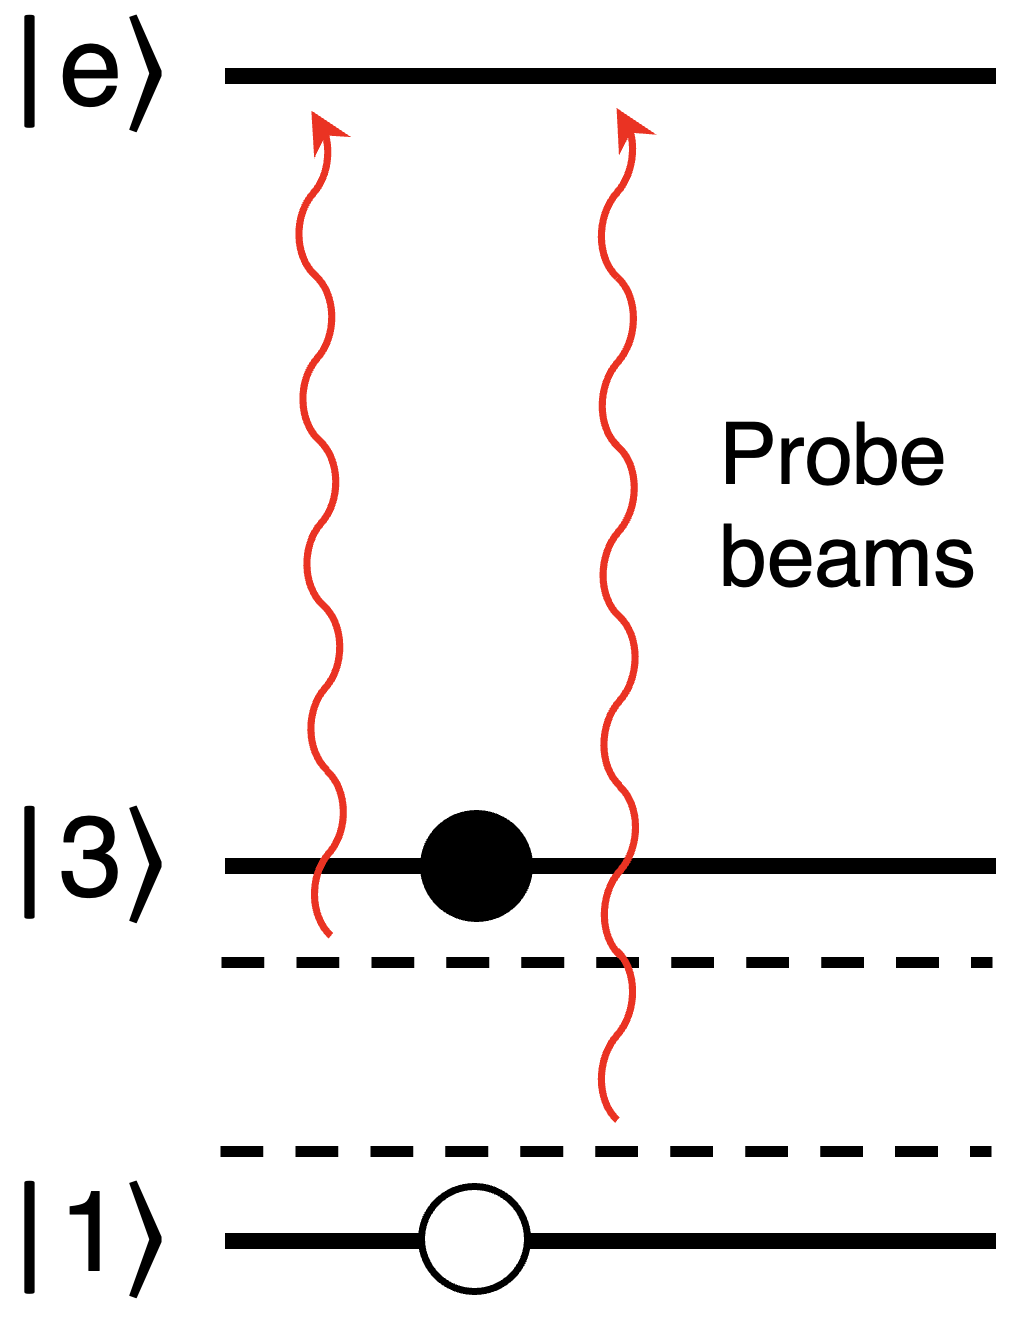
\includegraphics[width=0.8\textwidth]{figures_retreat/polrot_light_setup.png}
	\end{minipage}
	\hspace{-4.0cm}
	\begin{minipage}{0.15\textwidth}
		\centering
		\raisebox{-0.42\height}{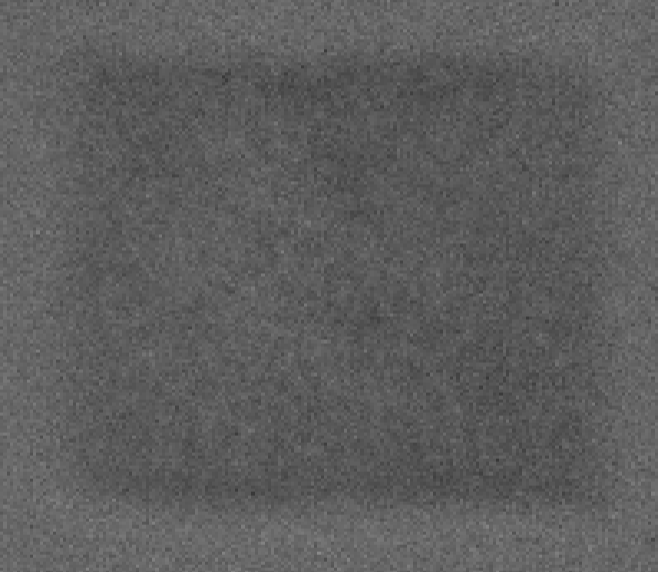
\includegraphics[width=0.6\textwidth]{figures_retreat/pr_box_B.png}}\\
		\vspace{1.5cm}
		\raisebox{-0.42\height}{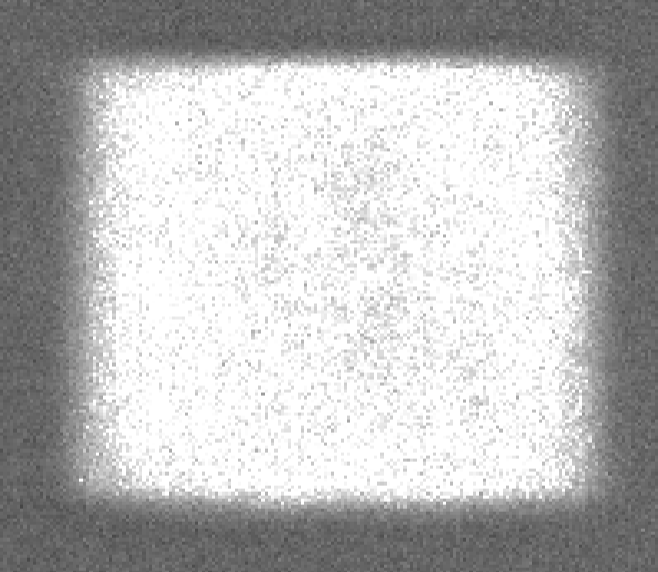
\includegraphics[width=0.6\textwidth]{figures_retreat/pr_box_A.png}}\\
	\end{minipage}
	
	\vspace{2.0cm}
	
	\begin{minipage}{0.28\textwidth}
		\flushleft
		\vspace{0.5cm}
		\textbf{Why not absorption imaging?}
		\vspace{0.5cm}
		\myfont
		\begin{minipage}{0.75\textwidth}
			\flushleft
			\vspace{1.0cm}
			\begin{itemize}				
				\item Resonant absorption imaging gives blacked out images for high-OD clouds
				
				\item Detuned absorption imaging results in distortions due to dispersive effects
				
				\item PRI gives better contrast with detuned imaging light
				
				\item PRI allows for higher imaging intensities for better S/N
			\end{itemize}
		\end{minipage}
	\end{minipage}
	\begin{minipage}{0.2\textwidth}
		\hspace{-7.7cm}
		\vspace{1.3cm}
		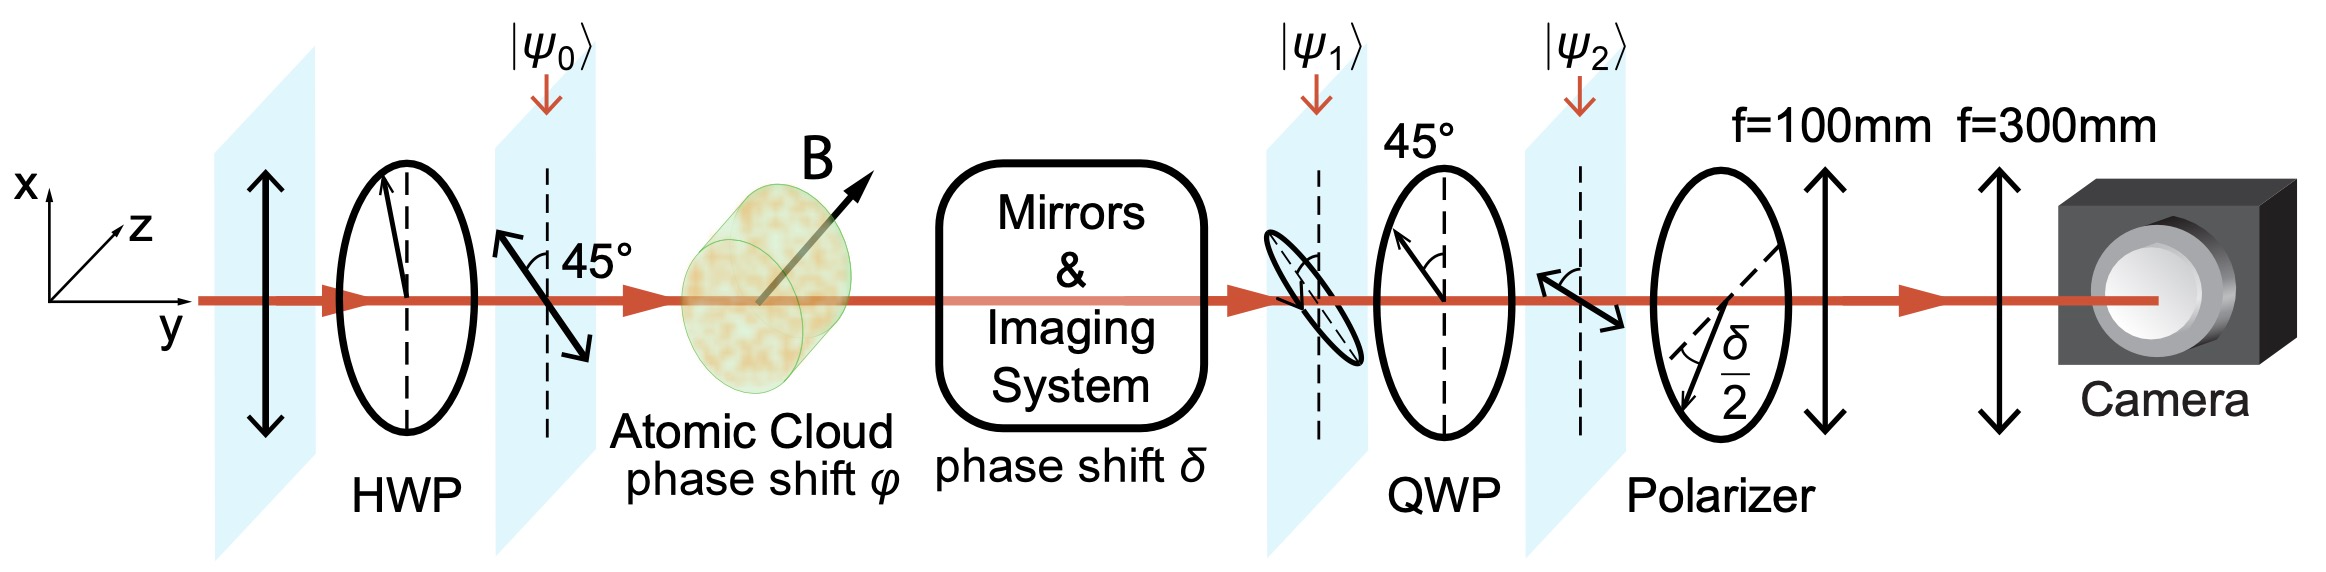
\includegraphics[width=1.75\textwidth]{figures_retreat/polrot_setup.png}\\
		\vspace{1.0cm}
		\hspace{-4.5cm}
		
\includegraphics[width=0.4\textwidth]{figures_retreat/box_abs_sound_A.png}
		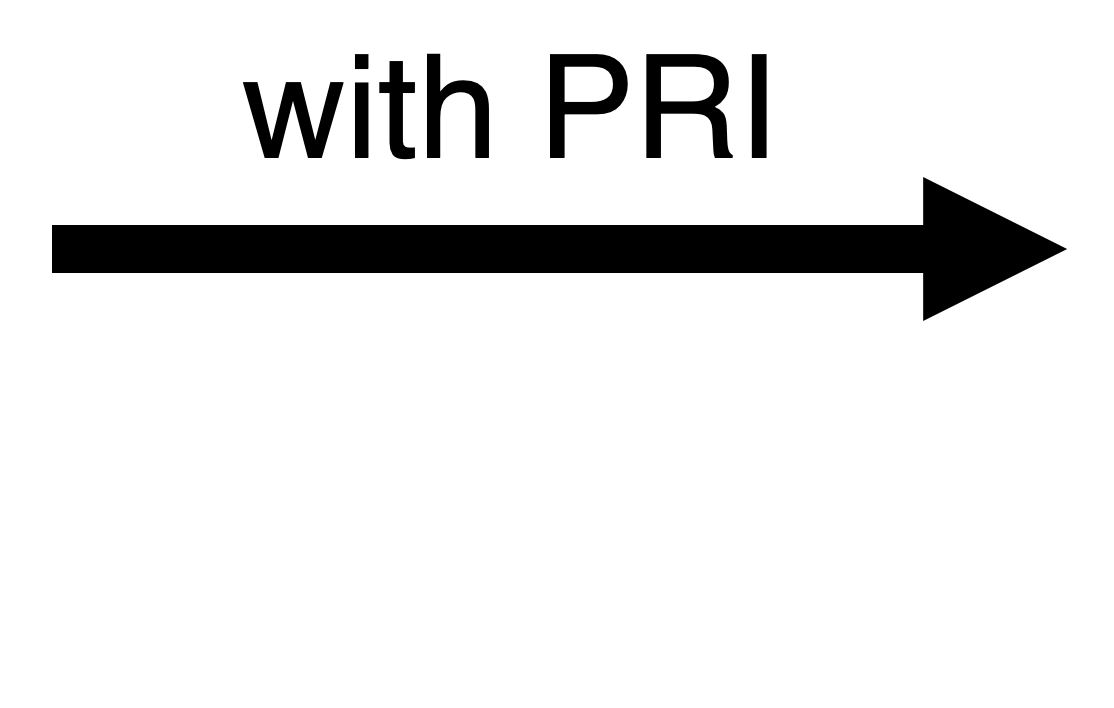
\includegraphics[width=0.4\textwidth]{figures_retreat/with_PRI.png}
		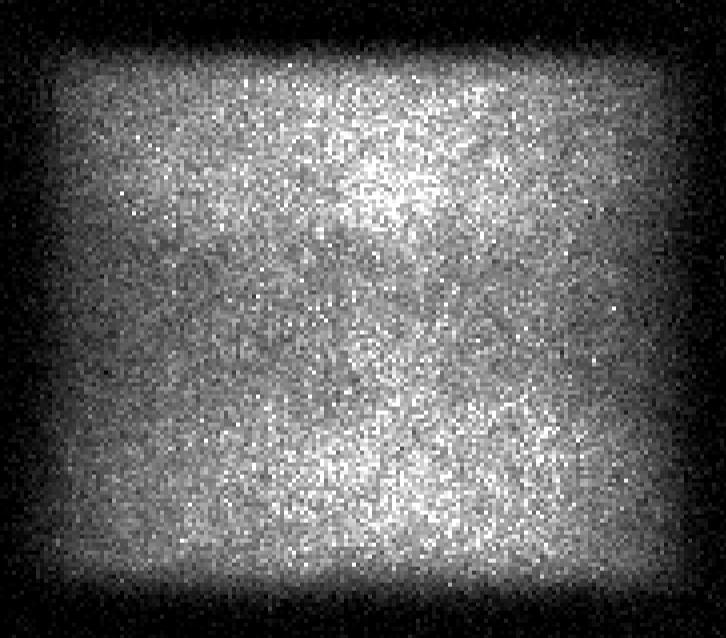
\includegraphics[width=0.4\textwidth]{figures_retreat/pr_sound_A.png}
	\end{minipage}	
	\vspace{-0.1cm}
	
}

	
	


\end{columns}



%% second row

\begin{columns} 
	
	%%%
	
	
	%%%%%%%%%%%%%%%%%%%%%%%%%%%%%%%%%%%%%%%%%%%%%
	
	\column{0.53} 
	\colorlet{blocktitlebgcolor}{BEC1grey}
	\block[roundedcorners=0]{\textcolor{BEC1blue}{Clogston-Chandrasekhar limit measurement}}
	{
		\begin{minipage}{0.20\textwidth}
			\flushleft
			\vspace{0.5cm}
			\textbf{Rapid Ramp procedure [2]}
			\vspace{0.5cm}
			\myfont
			\begin{itemize}
				\item A rapid B-field ramp to the BEC side adiabatically converts correlated pairs into molecules 
				\item Pair condensation after RR is (indirect) evidence for superfluidity in the box
											
			\end{itemize}
		\end{minipage}
		\hspace{2.0cm}
		\begin{minipage}{0.17\textwidth}
			\vspace{0.5cm}
			\hspace{1.0cm}
			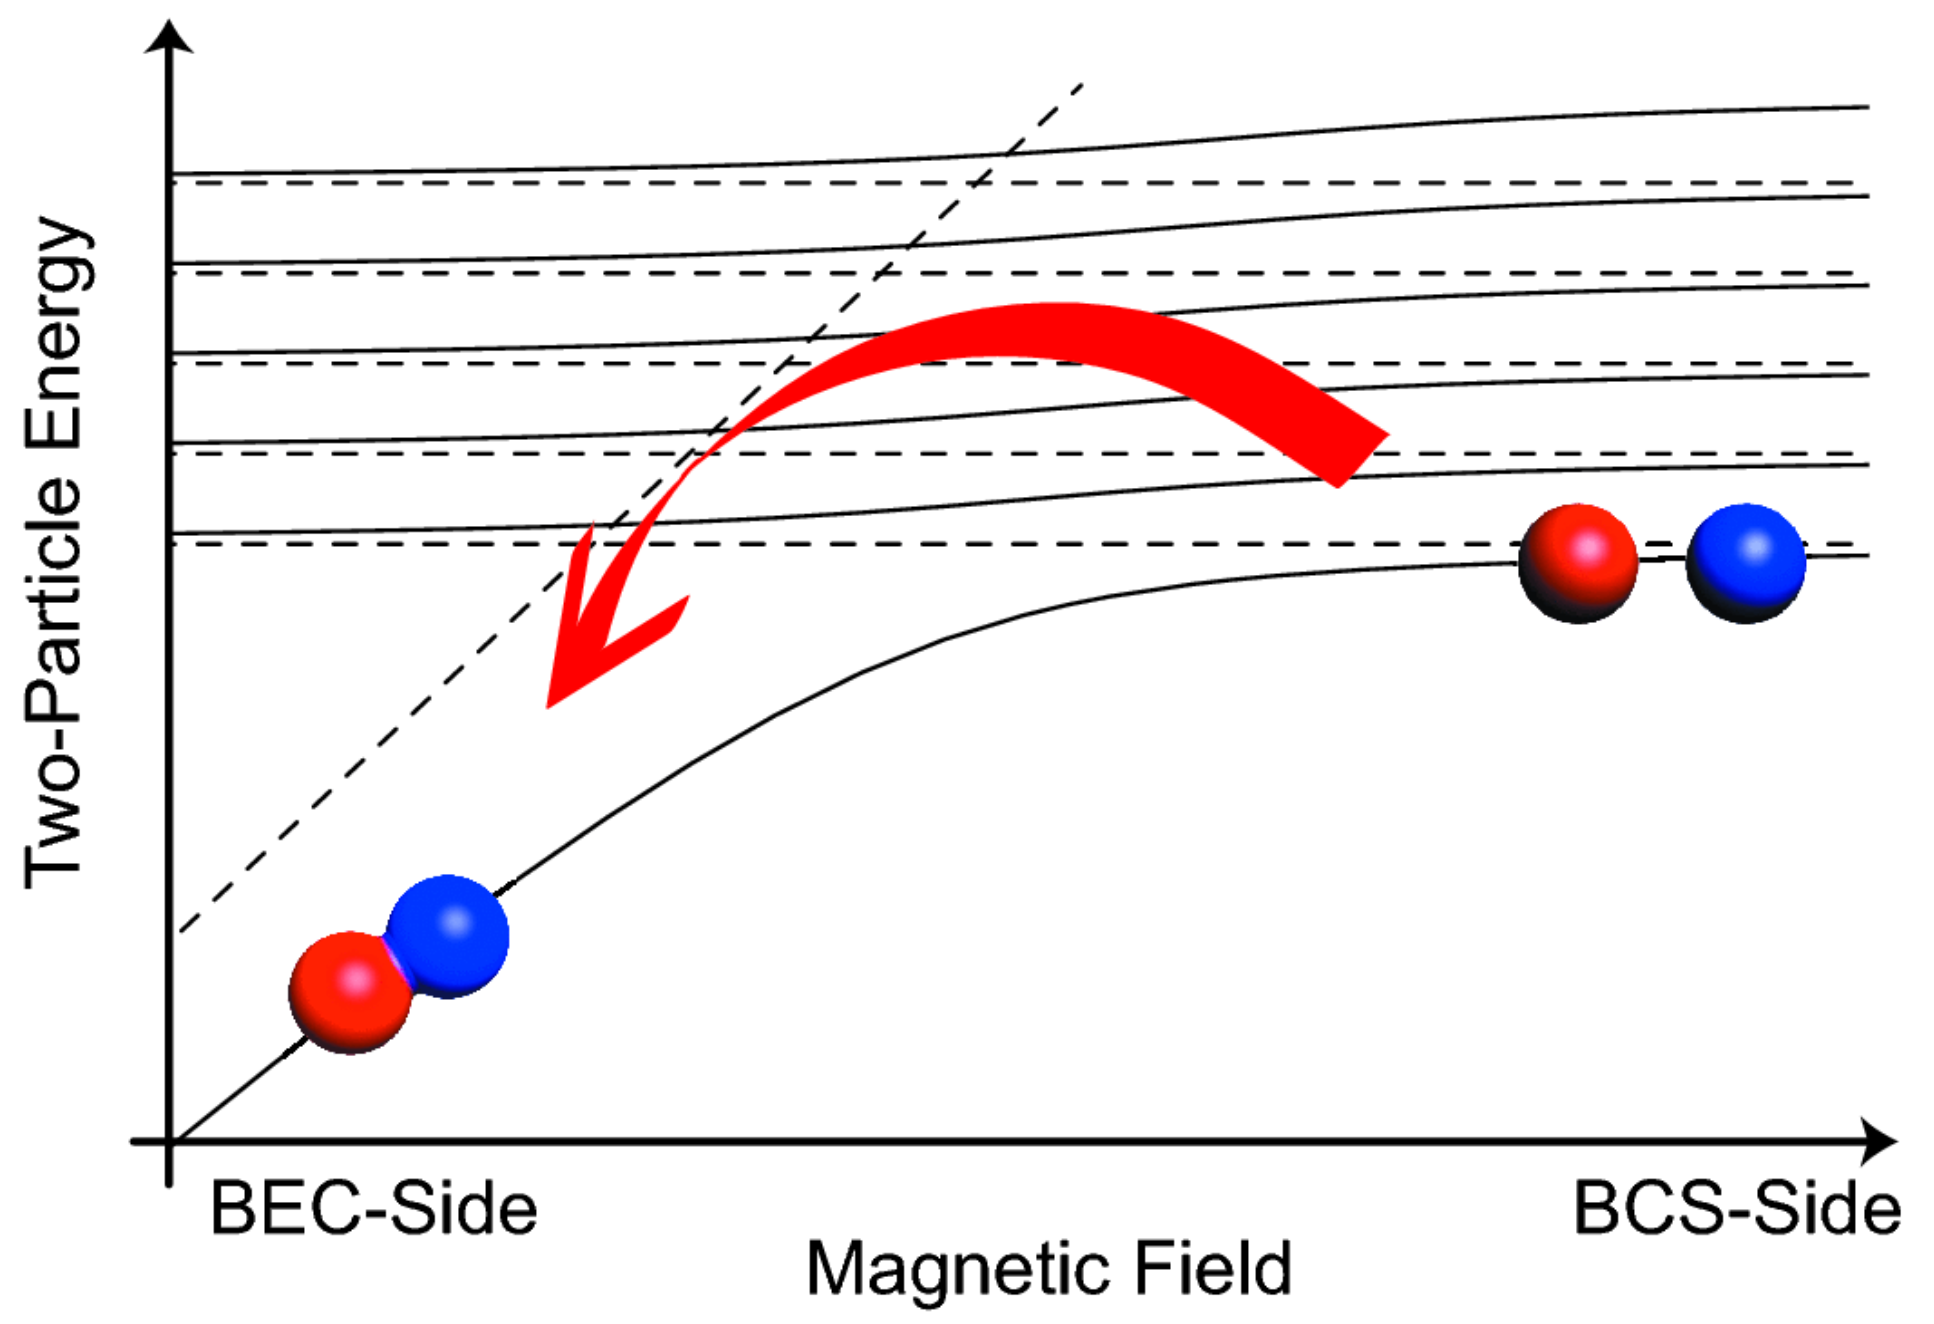
\includegraphics[width=1.1\textwidth]{figures_retreat/rapid_ramp.png}
		\end{minipage}
		\vspace{1.0cm}
		
		\begin{minipage}{0.5\textwidth}
			\hspace{3.0cm}
			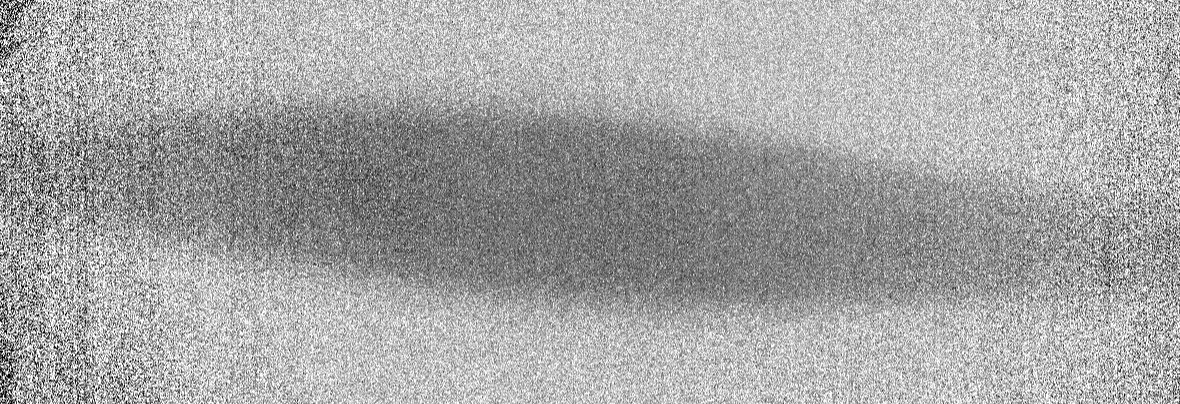
\includegraphics[width=0.35\textwidth]{figures_retreat/no_RR_TOF.png}
			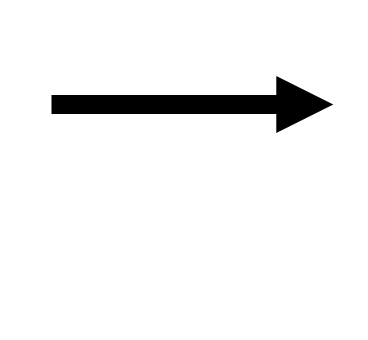
\includegraphics[width=0.1\textwidth]{figures_retreat/rightarrow.png}
			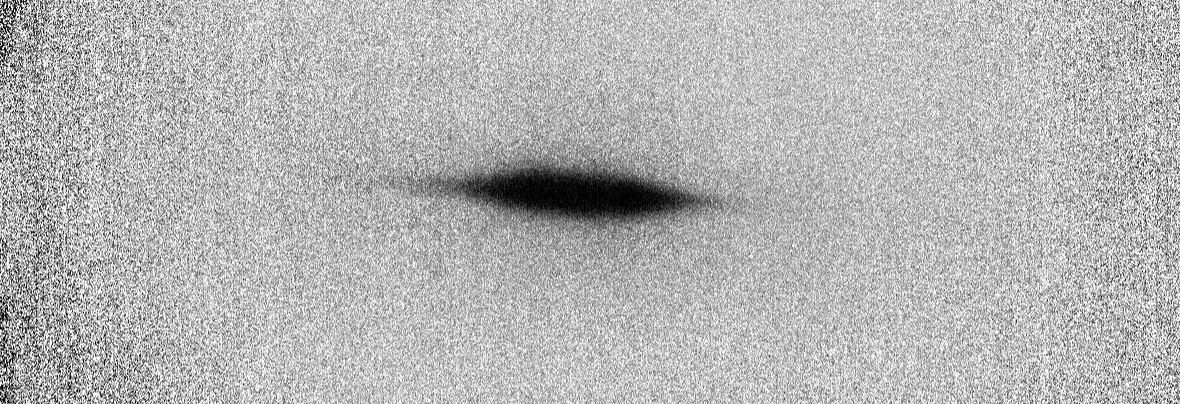
\includegraphics[width=0.35\textwidth]{figures_retreat/RR_TOF.png}
		\end{minipage}
		
		
		\vspace{2cm}
		\begin{minipage}{0.5\textwidth}
		\flushleft
		\textbf{Measuring the Clogston-Chandrasekhar limit}
		\vspace{0.5cm}
		\myfont
		\begin{minipage}{\textwidth}
			\flushleft
			\vspace{1.2cm}
			\begin{itemize}
				\item Clogston limit: Beyond a critical spin-imbalance, superfluidity is no longer supported
				\item Measured in harmonic trap [5], not yet in uniform trap
			\end{itemize}
		\end{minipage}
	\end{minipage}

		
	}
	
		
	\column{0.47} % See Section 4.4
	\colorlet{blocktitlebgcolor}{BEC1grey}
	\block[roundedcorners=0]{\textcolor{BEC1blue}{Outlook}}
	{
		\begin{minipage}{0.4\textwidth}
			\flushleft
			\textbf{First sound in spin-imbalanced system}
			\vspace{0.5cm}
			\myfont
			\begin{itemize}
				\item Sound with spin-imbalance? \textbf{Yes}
				\item How do hydrodynamic quantities change with spin-imbalance?
			\end{itemize}
		\end{minipage}
		
	\vspace{2.0cm}
	\begin{minipage}{0.4\textwidth}
		\hspace{1.0cm}
		\vspace{1.0cm}
		
\includegraphics[width=0.3\textwidth]{figures_retreat/box_abs_sound_A.png}
		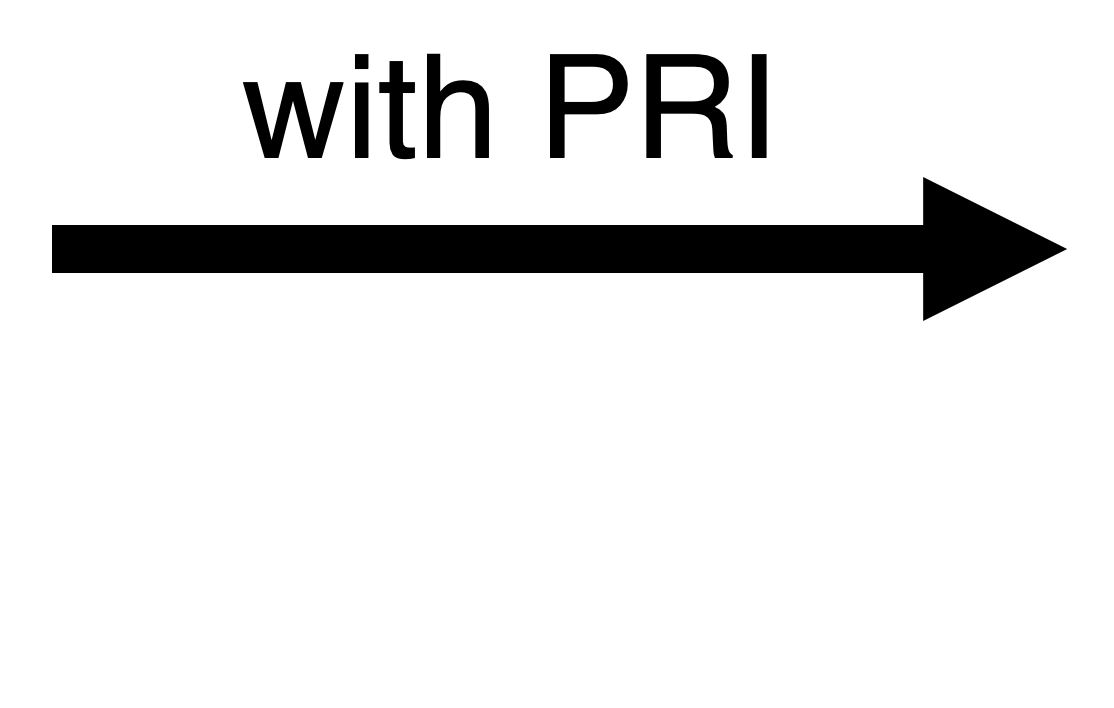
\includegraphics[width=0.3\textwidth]{figures_retreat/with_PRI.png}
		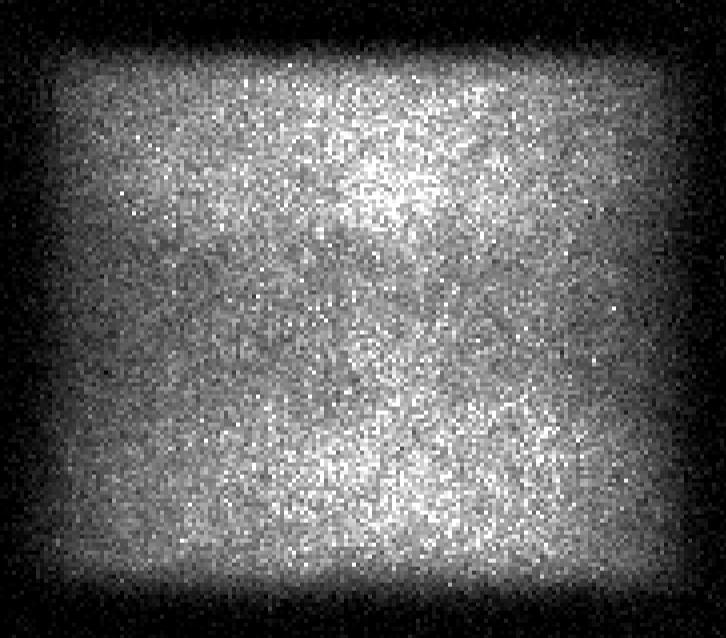
\includegraphics[width=0.3\textwidth]{figures_retreat/pr_sound_A.png}
	\end{minipage}	
	
	\vspace{1.0cm}
	\begin{minipage}{0.3\textwidth}
		\flushleft
		\textbf{Second sound in spin-imbalanced system}
		\vspace{0.5cm}
		\myfont
		\begin{itemize}
			\item Direct evidence for superfluidity in the box trap
			
			\item New transport phenomena?
		\end{itemize}		
	\end{minipage}
	\hspace{-4.0cm}
	\vspace{-1.0cm}
	\begin{minipage}{0.15\textwidth}
		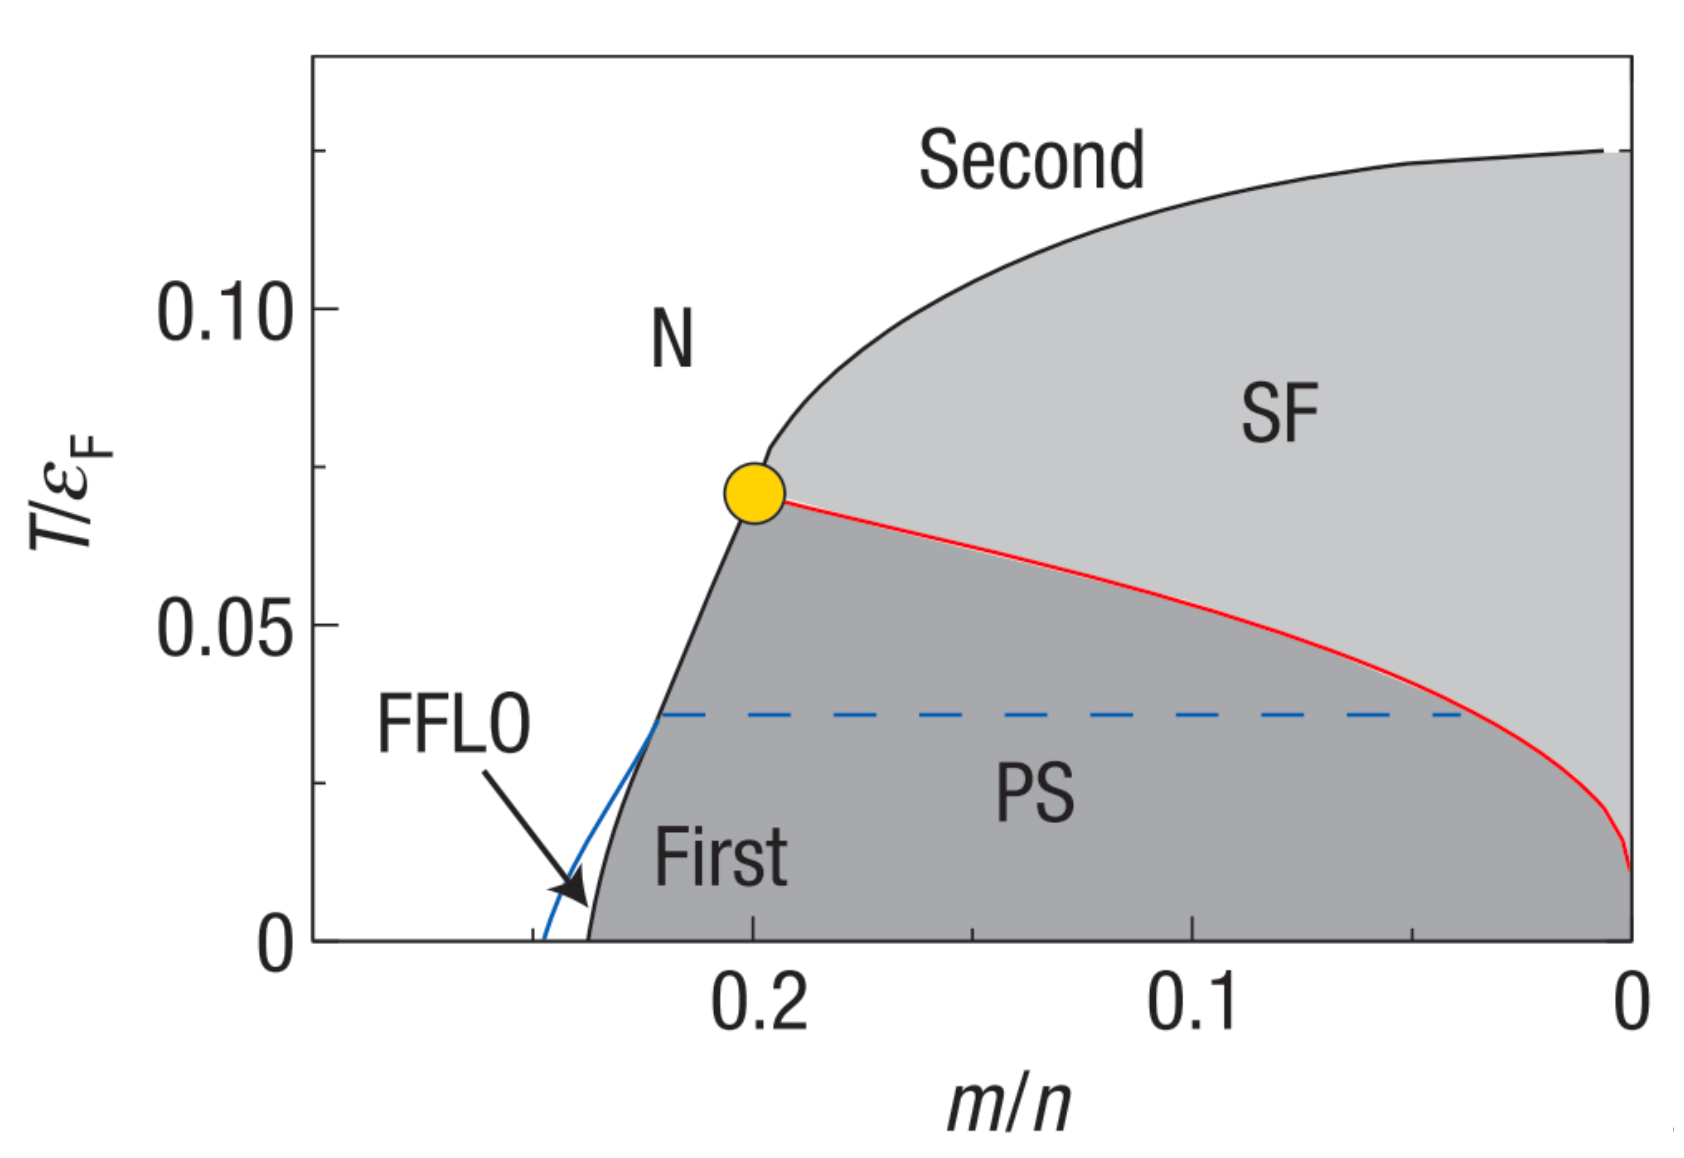
\includegraphics[width=\textwidth]{figures_retreat/FFLO_phase_diagram.png}
	\end{minipage}	
	
	
	\vspace{2.0cm}
	\begin{minipage}{0.25\textwidth}
		\flushleft
		\vspace{0.5cm}
		\textbf{Observing the FFLO state}
		\vspace{0.5cm}
		\myfont
		\begin{minipage}{0.75\textwidth}
			\flushleft
			\vspace{1.0cm}
			\begin{itemize}				
				\item Indirect evidence exists in 1D 
				\item Still elusive in 3D
			\end{itemize}
		\end{minipage}
	\end{minipage}
	\hspace{-8.2cm}
	\begin{minipage}{0.2\textwidth}
		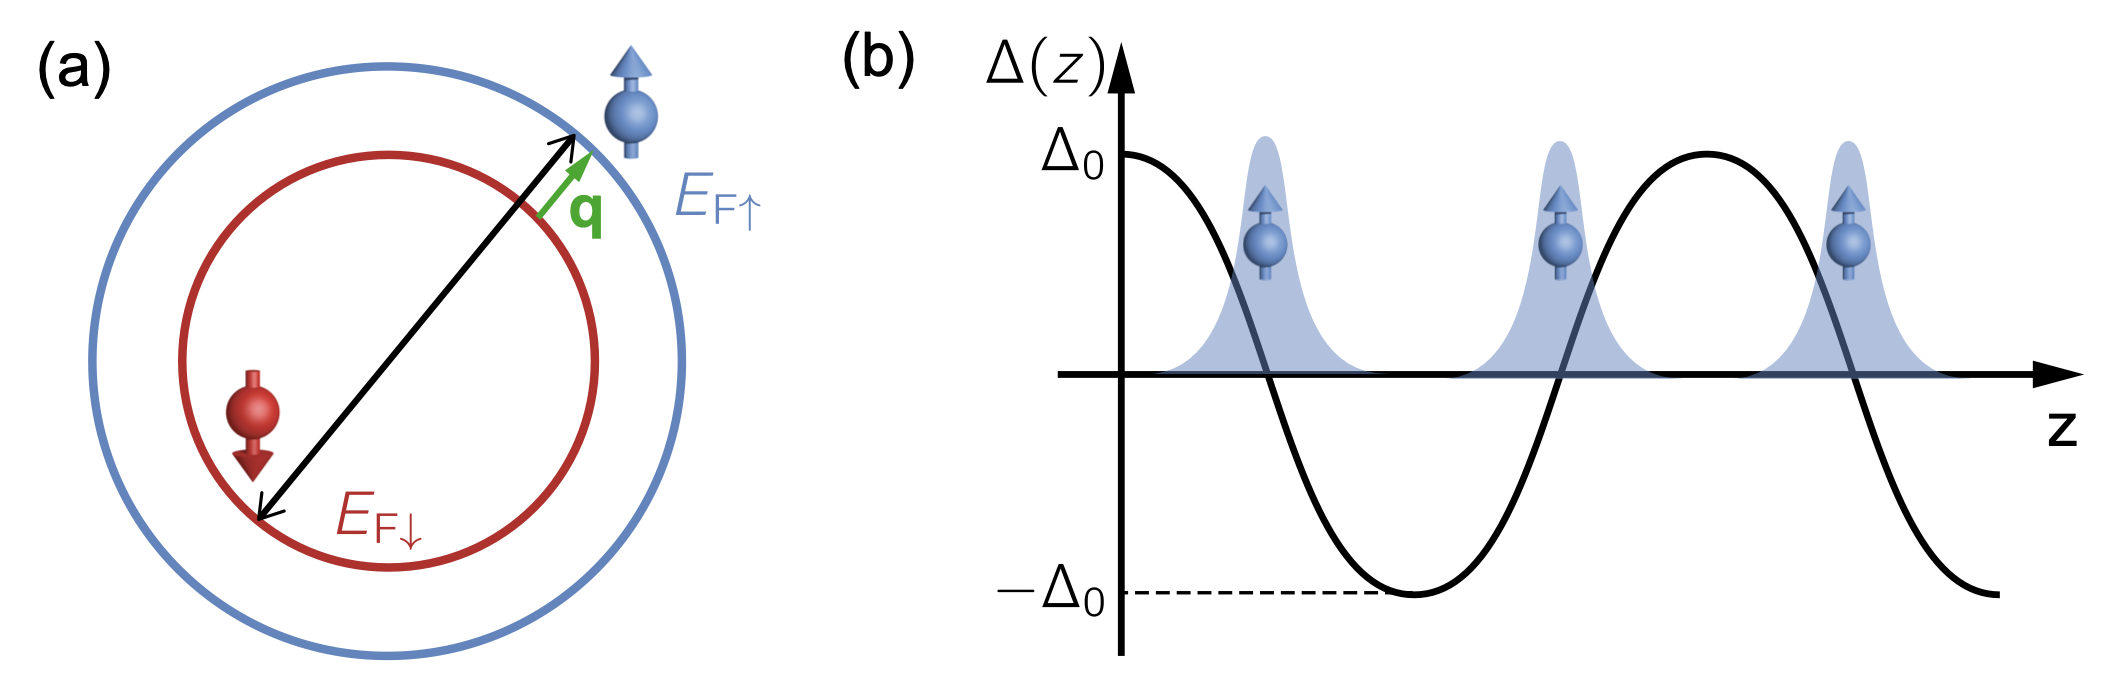
\includegraphics[width=1.3\textwidth]{figures_retreat/FFLO.png}
	\end{minipage}	
	\vspace{1.0cm}
	}
	\note[targetoffsetx=5cm, targetoffsety=-6.8cm, angle=0, radius=0cm,
	width=0.1cm, rotate=0, connection, linewidth=0cm,
	roundedcorners=0, innersep=0cm]{[6]}
	
	\note[targetoffsetx=5cm, targetoffsety=-15.8cm, angle=0, radius=0cm,
	width=0.1cm, rotate=0, connection, linewidth=0cm,
	roundedcorners=0, innersep=0cm]{[4]}
	
\end{columns}


\begin{columns} 
	\column{0.5}
	\colorlet{blocktitlebgcolor}{BEC1grey}
	\block[roundedcorners=0]{\textcolor{BEC1blue}{References}}
	{
	\begin{minipage}{0.2\textwidth}
		\myfont
		{[1]} B. Mukherjee et al., \textit{PRL}, 2017\\
		{[2]} M. W. Zwierlein, W. Ketterle,  \textit{La Rivista del Nuovo Cimento}, 2008\\
		{[3]} P. Patel, PhD Thesis, 2021 
	\end{minipage}
	\hspace{0.2cm}
	\begin{minipage}{0.2\textwidth}
		\myfont
		{[4]} Z. Yan, PhD Thesis, 2021\\
		{[5]} Shin, Yong-il, et al. \textit{Nature}, 2008\\
		{[6]} Partridge, G. B., et al., \textit{Science}, 2006
		{[7]} 
	\end{minipage}


	} 
	
	
	\column{0.5} 
	\colorlet{blocktitlebgcolor}{BEC1grey}
	\block[roundedcorners=0]{\textcolor{BEC1blue}{Funding}}{

	\begin{minipage}{0.24\textwidth}
	
\includegraphics[height=4.4cm]{Funding Logos/Air_Force_LogoAsset 16.png}
	\hspace{0.23cm}
	
\includegraphics[height=4.4cm]{Funding Logos/NSF_Logo.png}
	\hspace{0.23cm}
	
\includegraphics[height=4.4cm]{Funding Logos/Office_of_Naval_Research_Official_Logo.png}
	\end{minipage}
	\hspace{1.5cm}
	\begin{minipage}{0.19\textwidth}
	\myfont
	\flushleft
	AFOSR-MURI, National Science Foundation, Office of Naval Research, Vannevar Bush Faculty Fellowship
	\end{minipage}
	\vspace{0.29cm}
}
	
	
	

	
\end{columns}





\end{document}